\documentclass[11pt, twoside, reqno]{book}
\usepackage{amssymb, amsthm, amsmath, amsfonts}
\usepackage{graphicx}
\usepackage{amsrefs}
\usepackage{color}
\usepackage{hyperref}
\usepackage{verbatim}
\usepackage[title]{appendix}
\usepackage{pdfpages}

\usepackage{bardtex}

\styleoption{seniorproject}


\begin{document}

%For senior projects:
\titlepg{Don't Take This Personally: Sentiment Analysis for Identification of ``Subtweeting" on Twitter}{Noah Segal-Gould}
    {May}{2018}

\abstr

The Oxford English Dictionary states that ``subtweet" is defined as ``(on the social media application Twitter) a post that refers to a particular user without directly mentioning them, typically as a form of furtive mockery or criticism." Following the rapid growth and adoption of social networking websites like Twitter, sentiment analysis has garnered much research interest in recent years. To computationally identify and categorize opinions expressed in text, sentiment analysis of figurative language such as irony and sarcasm has garnered even more recent interest. In this project, I will treat the identification of subtweets as a figurative language sentiment analysis problem and apply a novel approach for data collection and labeling, as well as Naive Bayes text classification. By identifying subtweets as they are posted online in real time, I will create a Twitter bot which archives and interacts with them. In addition to the paper, this project will be made available online with its source code and all data collected during its completion.

\tableofcontents

\dedic

I dedicate this senior project to @jack, who has willfully made numerous changes to Twitter which inevitably angered millions.

\acknowl

Thank you professors Sven Anderson, Keith O'Hara, and Rebecca Thomas for making this project possible through your combined efforts to teach and advise me. Thank you Benjamin Sernau '17 for enduring through three years of Computer Science courses with me and being a source of unending joy in my life. Thank you to Julia Berry '18, Aaron Krapf '18, and Zoe Terhune '18 for being my very best friends and giving me things worth caring about. Finally, thank you to my parents Tammy Segal and Emily Taylor for your constant support and patience throughout my four years at Bard College. 

\startmain


\intro

\section{Background}
\label{background}

The news and social networking service Twitter had over 140 million active users who sent 340 million text-based Tweets to the platform every day by March of 2012 \cite{twitter_stats}. Since Twitter-founder Jack Dorsey sent the first Tweet in March of 2006 \cite{first_tweet} social scientists, advertisers, and computer scientists have applied machine learning techniques to understand the patterns and structures of the conversations held on the platform. One such technique is sentiment analysis, which seeks to ascertain the opinions of bodies of text. Sentiment analysis techniques are often treated as classification problems which seek to place text into categories such as \textbf{positive}, \textbf{negative}, and \textbf{neutral}.

On Twitter, the most common way to publicly communicate with another user is to compose a tweet and place an ``@" before the username of that user somewhere in the tweet (e.g. "How are you doing, @NoahSegalGould?"). Through this method, public discussions on Twitter maintain a kind of accountability: even if one were to miss the notification that they were mentioned in a tweet, one's own dashboard keeps a running list of their most recent mentions. 

If an individual sought to disparage or mock another, they could certainly do so directly. But the targeted user would probably notice, and through the search funtions of the platform, anyone could see who has mentioned either their own or another's username. Instead, a phenomenon persists in which users of the platform deliberately insult others in the vaguest way possible. Tweets of this kind are colloquially called ``subtweets" and typically target a specific person but do not contain the username of that person.

All users do not necessarily possess the same exact definition of ``subtweet." I trust the Oxford English Dictionary's ``[tweet] that refers to a particular user without directly mentioning them, typically as a form of furtive mockery or criticism," however that definition is perhaps too restrictive. Some individuals believe subtweets abide by this definition, but others expand it to allow inclusion of others' real names (especially if that individual does not own a Twitter account), and some do not even require that a particular user be the target of the tweet. In this project, I implement a classifier which abides by a particularly loose definition in order to please as many parties as possible. 

\section{Motivation}
\label{motivation_and_prior_work}

The inspiration for this project came from interests I garnered taking courses within Bard College's Computer Science department as well as its Experimental Humanities concentration. The very first course I attended at Bard College was Professor Keith O'Hara's \textit{Object-Oriented Programming with Robots}. It served as my first introduction to computer programming, and for my final project I created \textit{Fuzzfeed}: a Twitter bot which generated fake \textit{Buzzfeed} article titles. The following academic year, I wrote programs in Professor Collin Jennings' \textit{Signs and Symbols: Patter Recognition in Literature and Code} and Professor Rune Olsen's \textit{Cybergraphics} which analyzed and visualized topic models of poetry on Twitter. The first time I implemented sentiment analysis on my own was in Professor Gretta Tritch-Roman's \textit{Mapping the 19th Century City}, for which I sought to analyze 1860s New York City newspapers for their sentiments toward immigration. Natural language processing struck me as entertaining and fruitful, so I chose to pursue it further.

By my Junior year, my friends and I used Twitter on a daily basis. In my free time, I made Twitter bots that utilized Markov chains to generate text based on corpora of their tweets. Data collection became a passion of mine as I learned to appreciate the utility and acknowledge the deliberate limitations of web-based APIs. I taught myself web-scraping and utilized Python's \textit{BeautifulSoup} library to programmatically acquire text from Bard College's official online course catalog as well as Twitter's web interface. These skills for programmatically interacting with the world wide web became useful resources during the completion of this project.

My peers introduced me to subtweeting, and I started to pay closer attention to tweets that followed the typical patterns of distanced criticism that subtweets were known for. Because some format seemed to exist which was popularly applied to produce the optimal subtweet, I pitched the concept of subtweet classification to my senior project adviser, Professor Sven Anderson, and I started work on this project in the Fall.

I was initially motivated to complete a senior project on this topic because I wanted to create something useful to my peers and also challenge their notions of public and private interactions on social networking applications like Twitter. Individuals I knew personally would take to the platform to complain indirectly about one another through their subtweets. Friends and I shared evenings debating on if a particular mutual friend's complaints were actually subtweets, and I wondered if that guess-work could be done by a program. I also wanted to challenge the hypocrisy of utilizing a service which presents itself as a public forum to speak in distinctly private ways. Toward this end, I decided the project would be in pursuit of the following goals: it would provide a framework for collecting examples of subtweets, train a classification algorithm using those examples, and finally utilize that classifier in real time to make tweets which were intended to be unseen by specific parties easily accessible to all parties. In presenting covertly hurtful content as obviously hurtful in a public fashion, perhaps I could promote a particular awareness that tweets posted by public accounts were indeed publicly accessible, and that Twitter's End User License Agreement (EULA) allowed for this kind of monitoring.

\section{Changes in Data Acquisition}
\label{changes_in_data}

\section{Sentiment Analysis}
\label{sentiment_analysis}

Sentiment analysis and opinion mining are typically used synonymously. Both terms were apparently coined in 2003, respectively in "Sentiment Analysis: Capturing Favorability Using Natural Language Processing"\cite{sentiment_origin} and "Mining the Peanut Gallery: Opinion Extraction and Semantic Classification of Product Reviews"\cite{opinion_origin}. In a commercial context, sentiment analysis and opinion mining are useful tools for anyone looking to sell a product. With the vast social networks available, these methods are becoming widespread. Instead of focus groups, opinion polls, and conduct surveys, sentiment analysis and opinion mining programs are increasingly applied to social networking websites to analyze the sentiments and opinions of users toward topics and products. 

For various purposes, there exist numerous sentiment analysis and opinion mining methods. SemEval, which started as Senseval in 1998, holds evaluations in the form of competitions in which several tasks and subtasks are assigned. In 2015, SemEval tasks 10 \cite{SEMEVAL201510} and 11 \cite{SEMEVAL201511} focused respectively on sentiment analysis of figurative language on Twitter and sentiment analysis of Tweets in general. In 2016's task 4 \cite{SEMEVAL20164}, the focus was on sentiment analysis on Tweets, and again in 2017's task 4 \cite{SEMEVAL20174} it was the same with the added challenge of working with Arabic-only Tweets. The subtasks assigned within a particular task are used as problems to which anyone can send a submission as a solution. 

\section{The Twitter API}
\label{twitter_api}

\section{Regular Expressions, N-Grams, \& Tokenization}
\label{regular_expressions_etc}

\section{TF \& TF-IDF}
\label{tf_tf_idf}

TF-IDF, or term frequency-inverse document frequency, is a statistical representation of how important a single word is for each document in a collection of documents.

\section{Naive Bayes}
\label{naive_bayes}

Naive Bayes classifiers are probabilistic supervised learning models which make the "naive" assumption of independence between pairs of features being classified. Sentiment analysis is popularly performed through Naive Bayes.

\section{Statistical Considerations}
\label{statistical_considerations}

In tasks pertaining to text classification, like sentiment analysis, precision refers to the number of correctly labeled items which were labeled as belonging to the positive class and in fact did belong to that class (true positives) divided by the total number of elements which were labeled as belonging to the positive class including ones which were labeled positively either correctly or incorrectly. Recall, then, refers to the true positives divided by the total number of elements that actually belong to the positive class.

\chapter{Implementation}
\label{implementation}

\section{Searching for Tweets Using the Twitter API}
\label{searching_with_api}

\section{Cleaning the Data}
\label{cleaning_data}

\section{Training the Classifier \& K-Folds Cross-Validation}
\label{training_and_k_folds}

This is a process of splitting arrays into random train and test subsets according to Scikit Learn's \begin{verbatim}sklearn.model_selection.train_test_split\end{verbatim}

\chapter{Results}
\label{results}

\section{Distributions \& Datasets}
\label{distributions_and_datasets}

For this project, I acquired and combined two datasets: 

\begin{itemize}

\item Alec Go's Sentiment140 dataset \cite{GODATASET}. It features 1,600,000 4-point scale classified (\textbf{highly negative} to \textbf{highly positive}) Tweets. 800,000 of these Tweets are classified as \textbf{positive} and 800,000 of them are classified as \textbf{negative}. This dataset was not tagged by humans. Instead, it was based entirely on emoticons present within individual Tweets. 

\item Ibrahim Naji's dataset \cite{NAJIDATASET}, which features 1,578,628 Tweets. 790,185 of these Tweets are classified as \textbf{positive} and 788,443 of these Tweets are classified as \textbf{negative}. It was tagged by humans and on a binary (either \textbf{negative} or \textbf{positive}) scale.

\end{itemize}

\section{Confusion Matrices}
\label{confusion_matrices}

A confusion matrix is a table which visualizes the performance of an algorithm. In this case, I implemented a Naive Bayes classifier from Scikit Learn on my dataset and included in my results is a confusion matrix of the performance:

\section{Most Informative Features}
\label{most_informative_features}

\section{Statistical Analysis}
\label{statistical_analysis}

\chapter{Conclusion}
\label{conclusion}

\section{The Twitter Bot}
\label{the_twitter_bot}

\section{Summary of Project Achievements}
\label{summary}

\section{Future Work \& Considerations}
\label{future_work_and_considerations}

\begin{bibliog}

\bib{twitter_stats}{article}{
author = {Twitter Inc.},
title = {Twitter turns six},
eprint = {https://blog.twitter.com/official/en_us/a/2012/twitter-turns-six.html}
date = {2012}
}

\bib{first_tweet}{article}{
author = {Dorsey, Jack}
title = {inviting coworkers},
eprint = {https://twitter.com/jack/status/29}
date = {2006}
}

\bib{twitter_ibm}{article}{
author = {Alexander, Forsyth}
title = {How to use Twitter activity to measure the effectiveness of your marketing},
eprint = {https://www.ibm.com/blogs/business-analytics/how-to-use-twitter-activity-to-measure-the-effectiveness-of-your-marketing/}
date = {2016}
}

\bib{politics_sentiment_analysis}{article}{
author = {Wang, Hao},
author = {Can, Dogan},
author = {Kazemzadeh, Abe},
author = {Bar, Fran\c{c}ois},
author = {Narayanan, Shrikanth}
title = {A System for Real-time Twitter Sentiment Analysis of 2012 U.S. Presidential Election Cycle},
journal = {Proceedings of the ACL 2012 System Demonstrations},
volume = {ACL '12},
date = {2012},
pages = {115--120}
}

\bib{hateful_conduct_policy}{article}{
author = {Twitter Inc.},
title = {Hateful conduct policy},
eprint = {https://help.twitter.com/en/rules-and-policies/hateful-conduct-policy}
}

\bib{sentiment_origin}{article}{
author = {Nasukawa, Tetsuya},
author = {Yi, Jeonghee},
title = {Sentiment Analysis: Capturing Favorability Using Natural Language Processing},
journal = {Proceedings of the 2nd International Conference on Knowledge Capture},
eprint = {http://doi.acm.org/10.1145/945645.945658},
volume = {K-CAP '03},
pages = {70--77},
date = {2003}
}

\bib{opinion_origin}{article}{
author = {Dave, Kushal},
author = {Lawrence, Steve},
author = {Pennock, David M.},
title = {Mining the Peanut Gallery: Opinion Extraction and Semantic Classification of Product Reviews},
journal = {Proceedings of the 12th International Conference on World Wide Web},
eprint = {http://doi.acm.org/10.1145/775152.775226},
volume = {WWW '03},
pages = {519--528},
date = {2003}
}

\bib{SEMEVAL201510}{article}{
title = {SemEval-2015 Task 10: Sentiment Analysis in Twitter},
author = {Rosenthal, Sara},
author = {Nakov, Preslav},
author = {Kiritchenko, Svetlana},
author = {Mohammad, Saif},
author = {Ritter, Alan},
author = {Stoyanov, Veselin},
journal = {SemEval@ NAACL-HLT},
pages={451--463},
date={2015}
}

\bib{SEMEVAL201511}{article}{
title = {SemEval-2015 Task 11: Sentiment Analysis of Figurative Language in Twitter},
author = {Ghosh, Aniruddha},
author = {Li, Guofu},
author = {Veale, Tony},
author = {Rosso, Paolo},
author = {Shutova, Ekaterina},
author = {Barnden, John},
author = {Reyes, Antonio},
journal = {Proceedings of the 9th International Workshop on Semantic Evaluation (SemEval 2015)},
pages={470--478},
date={2015}
}

\bib{SEMEVAL20164}{article}{
title = {SemEval-2016 Task 4: Sentiment Analysis in Twitter},
author = {Nakov, Preslav},
author = {Ritter, Alan},
author = {Rosenthal, Sara},
author = {Sebastiani, Fabrizio},
author = {Stoyanov, Veselin},
journal = {SemEval@ NAACL-HLT},
pages = {1--18},
date = {2016}
}

\bib{SEMEVAL20174}{article}{
title = {SemEval-2017 Task 4: Sentiment Analysis in Twitter},
author = {Rosenthal, Sara},
author = {Farra, Noura},
author = {Nakov, Preslav},
journal = {Proceedings of the 11th International Workshop on Semantic Evaluation (SemEval-2017)},
pages = {502--518},
date = {2017}
}

\bib{GODATASET}{article}{
title = {Twitter Sentiment Classification using Distant Supervision},
author = {Go, Alec},
author = {Bhayani, Richa},
author = {Huang, Lei},
journal = {CS224N Project Report, Stanford},
pages = {12},
date = {2009}
}

\bib{NAJIDATASET}{article}{
title = {Twitter Sentiment Analysis Training Corpus (Dataset)},
author = {Naji, Ibrahim},
eprint = {http://thinknook.com/twitter-sentiment-analysis-training-corpus-dataset-2012-09-22/},
date={2013}
}

\end{bibliog}

\begin{appendices}
	
\chapter{Classifier Creator Program}
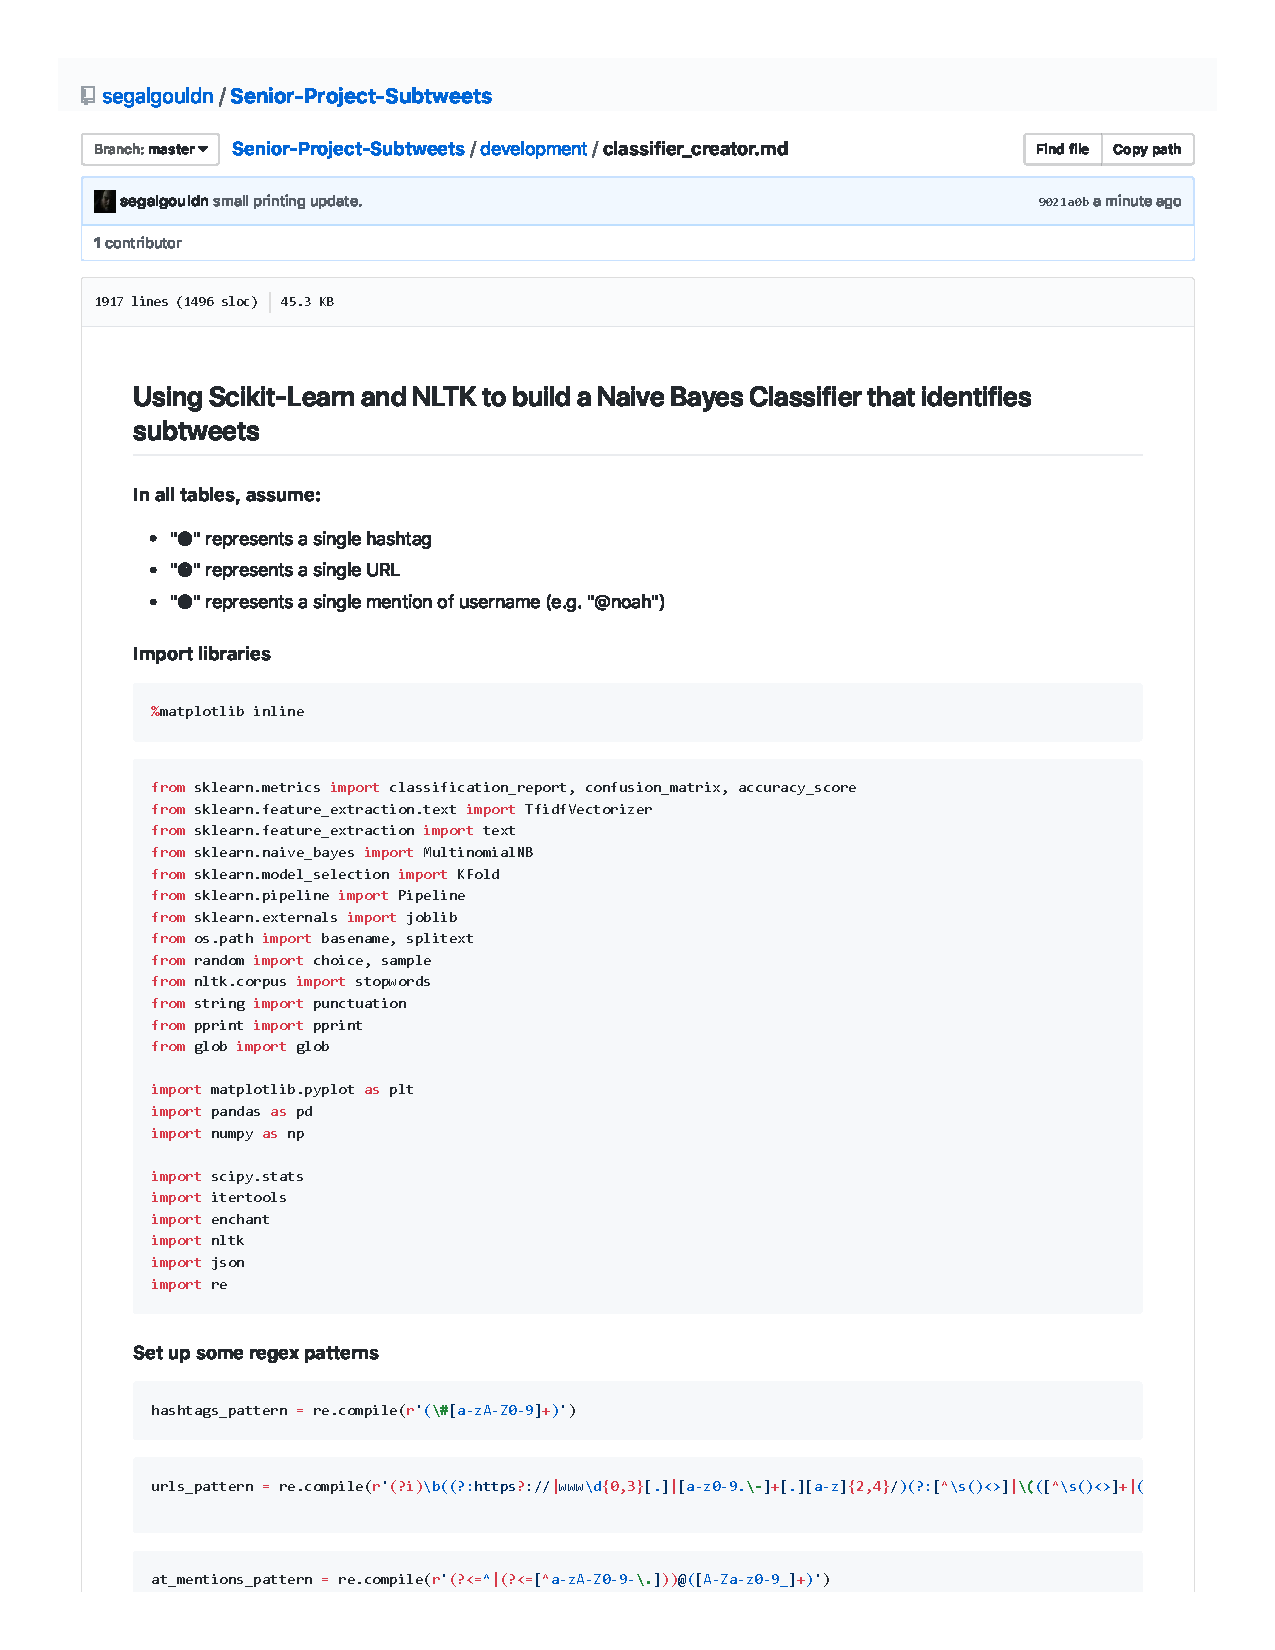
\includepdf[pages=-]{../classifier_creator.pdf}

\end{appendices}

\end{document}

% end of file bardproj_template.tex
